\section{Machine Learning}
\label{sec:ml}
%% Definition

For the past decades, Machine Learning (ML) has become one of the most powerful tools, allowing individuals to perform complex analyses for better insights. It has been bringing significant benefits in various vital fields, such as business, healthcare, agriculture or traffic management, etc.

The term "Machine Learning" was popularized in 1959 by Arthur Samuel \cite{samuel2000gameofcheckers}. He defined ML as "the field of study that gives computers the ability to learn without being explicitly programmed". In 1997, Mitchell \cite{mitchell1997machine} provided the definition “A computer program is said to learn from experience E with respect to some class of tasks T and performance measure P, if its performance at tasks in T, as measured by P, improves with experience E”. In other words, ML can be explained as automating and improving the learning process of computers based on their experiences without being actually programmed i.e. without any human assistance.

In the area of big data, ML derives insightful information from large volumes of data by leveraging algorithms to identify patterns and learn in an iterative process. The system applies some transformations to the input data to extract frequent or special patterns, which are usually called features, then uses them to predict the output. The performance is then evaluated by appropriate metrics for the given task. Based on these scores, the system can choose the best transformation for each problem among a set of predefined functions (also known as hypothesis space). 

In general, machine learning algorithms are divided into three common types: supervised learning, unsupervised learning, and reinforcement learning. 

\begin{itemize}
    
%% Supervised learning
\item  \textbf{Supervised learning} \cite{goodfellow2016deep}: Supervised learning is when the model getting trained on a labeled dataset, which allows the model to learn and grow more accurate over time. A labeled dataset is one that has both input and output parameters. Supervised machine learning is the mostly-used type today.

\begin{figure}[!h]
    \centering
    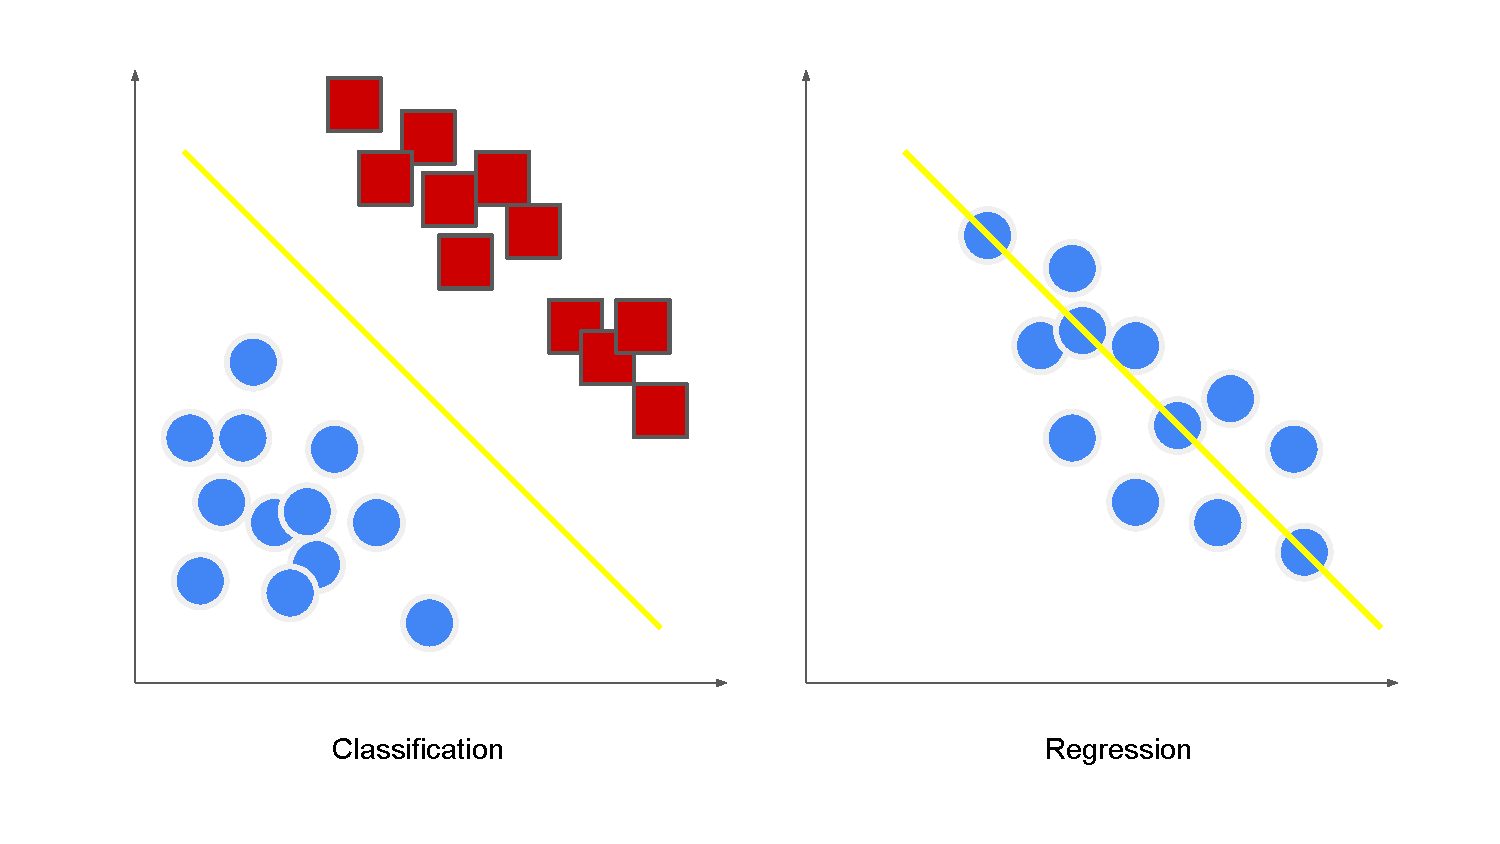
\includegraphics[width=\textwidth]{content/resources/new_images/related_works/supervised.pdf}
    \caption{Classification task and regression task}
    \label{fig:supervised}
\end{figure}

Two common types of supervised learning algorithms are classification and regression. Classification is the task of assigning the data into multiple categorical classes. For example, an algorithm would be trained with pictures of dogs and cats, all labeled by humans, and the machine would learn ways to identify pictures of dogs or cats on its own.
Meanwhile, regression is the task of distinguishing the data into continuous real values. Examples of this type of task include predicting the house prices from their properties or predicting the age of people based on their face image. Figure \ref{fig:supervised} demonstrates the difference between the two tasks.

% Unsupervised learning
 
\item  \textbf{Unsupervised learning} \cite{goodfellow2016deep}: The technique analyzes and clusters unlabeled datasets using machine learning algorithms. These algorithms find hidden patterns and data without any human intervention, i.e., we don’t give output to our model. The training model has only input parameter values and it can group unsorted information according to similarities, patterns and differences without any prior training of data.

Two common unsupervised learning algorithms are clustering and association. Clustering techniques are applied to group data based on different patterns that our machine model finds, such as similarities or differences, whereas association rule learning is a rule-based ML technique that finds out some very useful relations between parameters of the large portions of data.
 
Figure \ref{fig:unsupervised} depicts two use cases of unsupervised learning. Clustering can be used to segment customers based on their distinct attributes and association can help suggesting what customers should buy based on  what others have bought.
 
 \begin{figure}[!h]
     \centering
     \begin{subfigure}
         \centering
         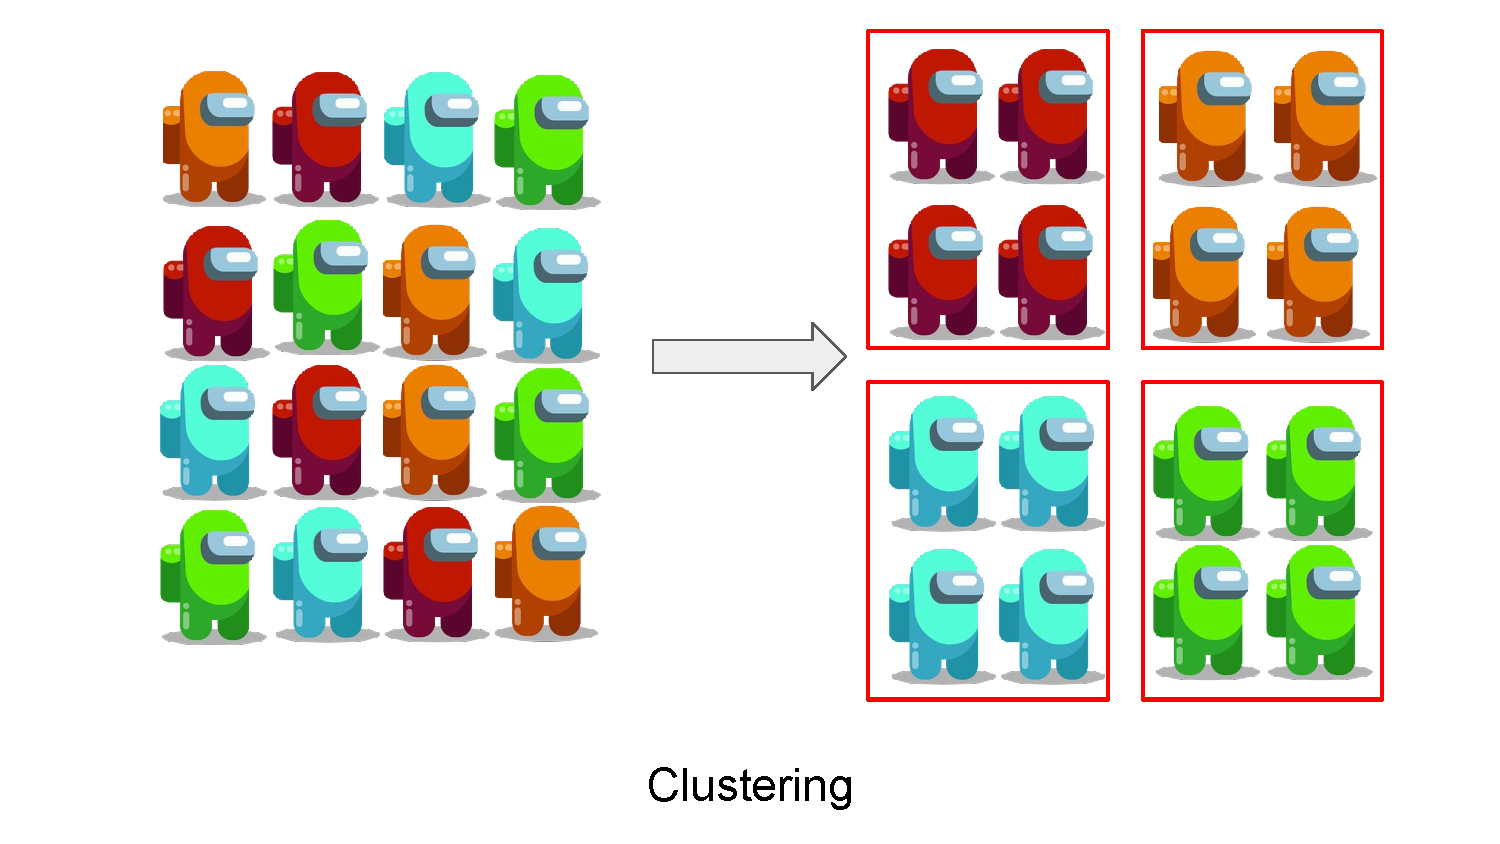
\includegraphics[width=0.45\textwidth]{content/resources/new_images/related_works/clustering.pdf}
     \end{subfigure}
     \hfill
     \begin{subfigure}
         \centering
         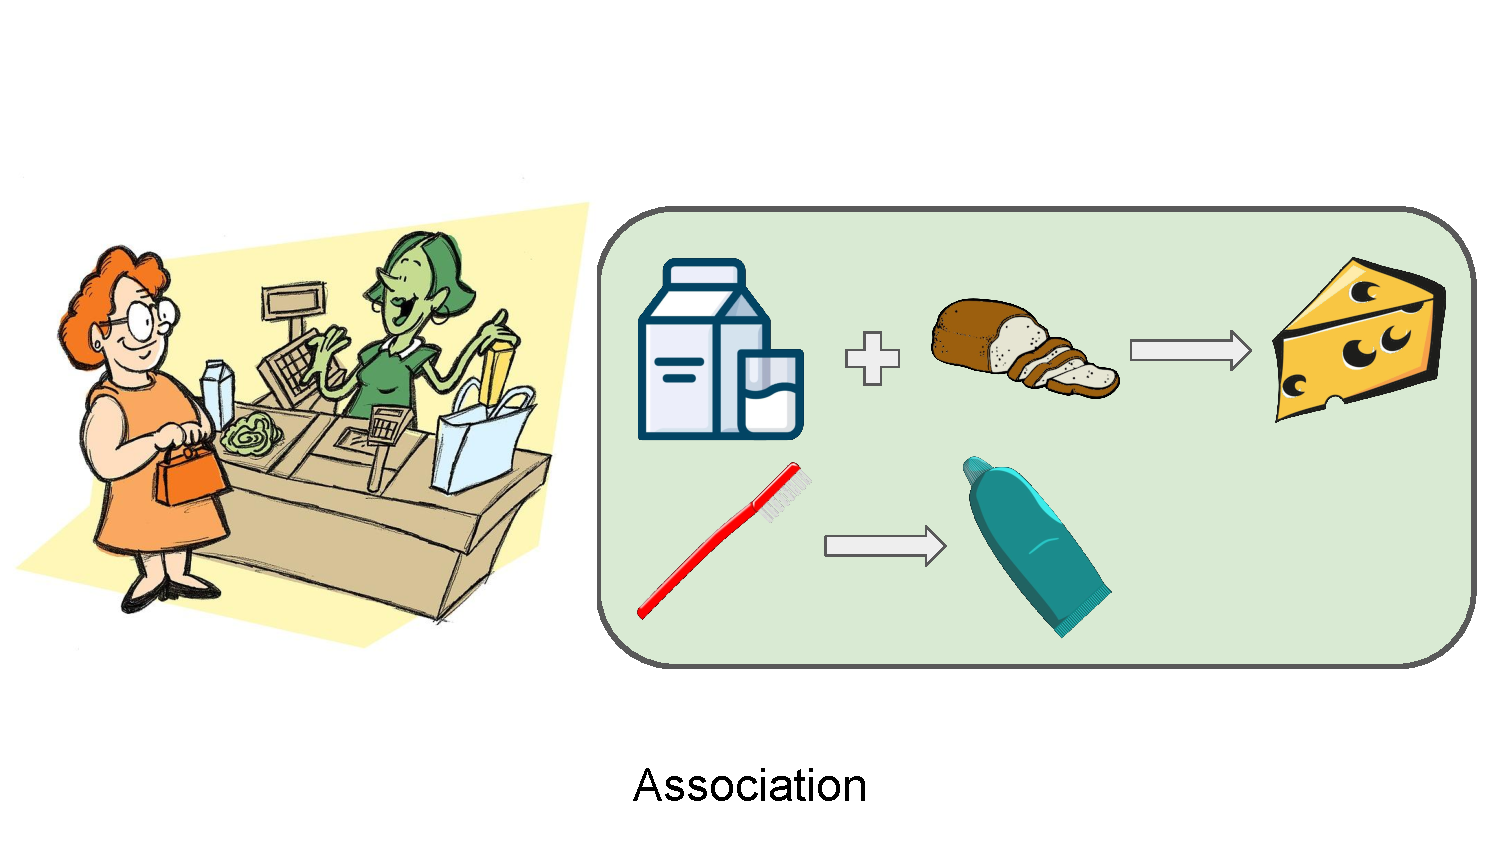
\includegraphics[width=0.45\textwidth]{content/resources/new_images/related_works/association.pdf}
     \end{subfigure}
        \caption{Clustering task and Association task}
        \label{fig:unsupervised}
\end{figure}

 
 
 % Reinforcement learning
 
 \item \textbf{Reinforcement learning} \cite{sutton1998introduction}: In this technique, the model (or the agent) learns the behavior or pattern by interacting with the environment and assessing the reward to increase its performance. The main goal of the agent is to take action in order to maximize the notion of cumulative reward.
 Reinforcement learning differs from supervised learning in not needing labeled input/output pairs to be presented, and in not needing sub-optimal actions to be explicitly corrected. These algorithms are specific to a particular problem e.g. Google Self Driving car \cite{jain2013google}, AlphaGo \cite{silver2016mastering} where a bot competes with humans and even itself to get better and better performers in Go Game. Each time we feed in data, they learn and add the data to their knowledge. So, the more it learns the better it gets trained and hence experienced. 
 
 Looking at the Figure \ref{fig:reinforcement}, the agent is assigned a mission to obtain the reward while minimizing the path cost. Each time it reaches the reward, it learns a new behaviour and optimize its own path for the following iteration. 
 
\begin{figure}[!h]
    \centering
    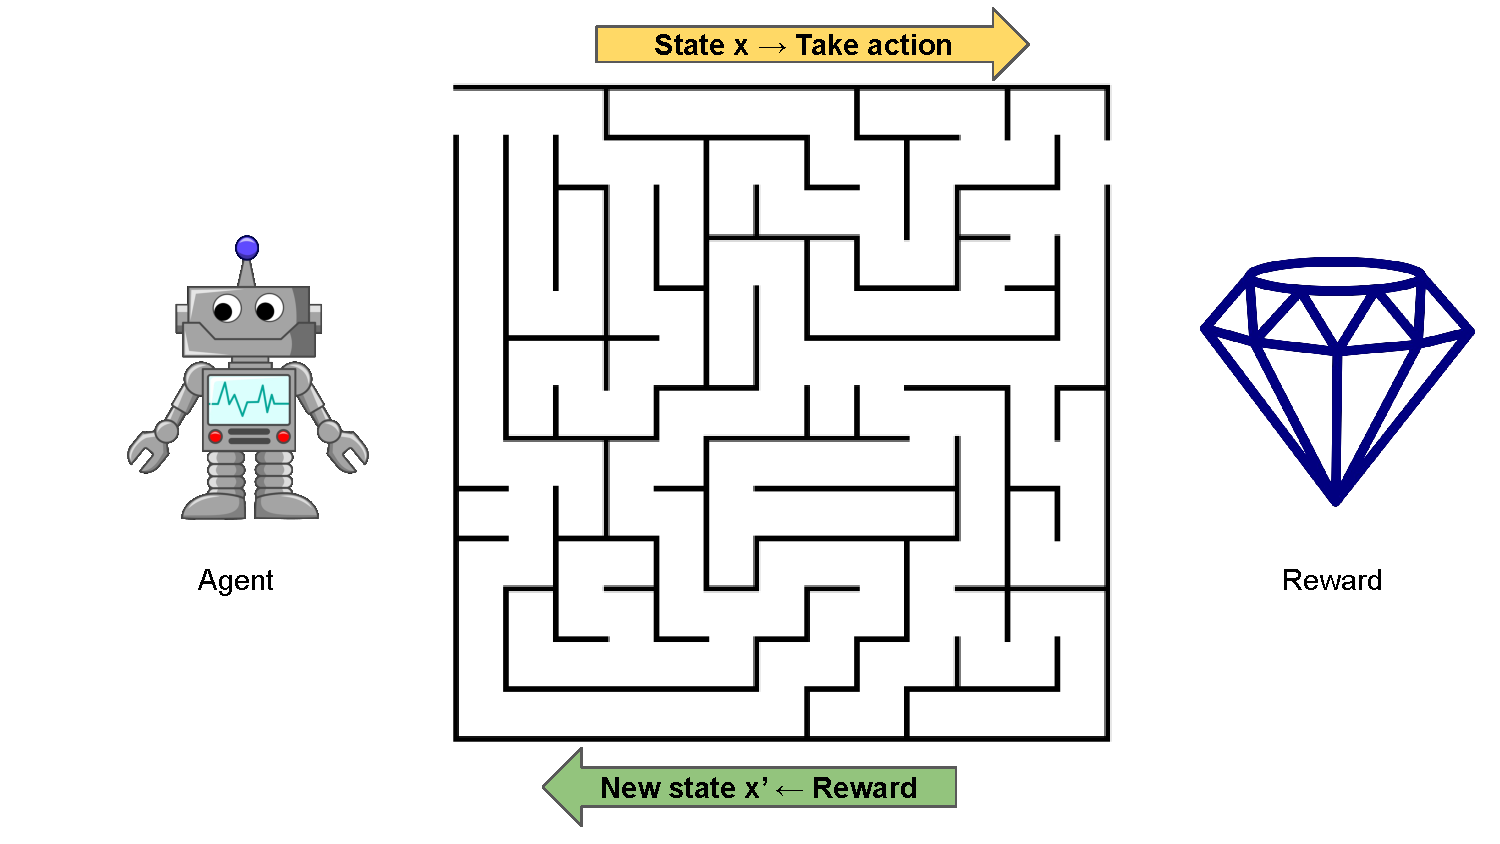
\includegraphics[width=\textwidth]{content/resources/new_images/related_works/reinforcement.pdf}
    \caption{An example for Reinforcement learning. The agent is tasked to acquire the reward while searching for the most optimized track.}
    \label{fig:reinforcement}
\end{figure}
 
 \end{itemize}



